% mnras_template.tex
%
% LaTeX template for creating an MNRAS paper
%
% v3.0 released 14 May 2015
% (version numbers match those of mnras.cls)
%
% Copyright (C) Royal Astronomical Society 2015
% Authors:
% Keith T. Smith (Royal Astronomical Society)

% Change log
%
% v3.0 May 2015
%    Renamed to match the new package name
%    Version number matches mnras.cls
%    A few minor tweaks to wording
% v1.0 September 2013
%    Beta testing only - never publicly released
%    First version: a simple (ish) template for creating an MNRAS paper

%%%%%%%%%%%%%%%%%%%%%%%%%%%%%%%%%%%%%%%%%%%%%%%%%%
% Basic setup. Most papers should leave these options alone.
\documentclass[fleqn,usenatbib]{mnras}

% MNRAS is set in Times font. If you don't have this installed (most LaTeX
% installations will be fine) or prefer the old Computer Modern fonts, comment
% out the following line
\usepackage{newtxtext,newtxmath}
% Depending on your LaTeX fonts installation, you might get better results with one of these:
% \usepackage{mathptmx}
% \usepackage{txfonts}

% Use vector fonts, so it zooms properly in on-screen viewing software
% Don't change these lines unless you know what you are doing
\usepackage[T1]{fontenc}

% Allow "Thomas van Noord" and "Simon de Laguarde" and alike to be sorted by "N" and "L" etc. in the bibliography.
% Write the name in the bibliography as "\VAN{Noord}{Van}{van} Noord, Thomas"
\DeclareRobustCommand{\VAN}[3]{#2}
\let\VANthebibliography\thebibliography
\def\thebibliography{\DeclareRobustCommand{\VAN}[3]{##3}\VANthebibliography}


%%%%% AUTHORS - PLACE YOUR OWN PACKAGES HERE %%%%%

% Only include extra packages if you really need them. Common packages are:
\usepackage{graphicx}	% Including figure files
\usepackage{amsmath}	% Advanced maths commands
% \usepackage{amssymb}	% [CHANGED] Extra maths symbols
\usepackage{anyfontsize} % [ADDED] Allow any font size

%%%%%%%%%%%%%%%%%%%%%%%%%%%%%%%%%%%%%%%%%%%%%%%%%%

%%%%% AUTHORS - PLACE YOUR OWN COMMANDS HERE %%%%%

% Please keep new commands to a minimum, and use \newcommand not \def to avoid
% overwriting existing commands. Example:
%\newcommand{\pcm}{\,cm$^{-2}$}	% per cm-squared

%%%%%%%%%%%%%%%%%%%%%%%%%%%%%%%%%%%%%%%%%%%%%%%%%%

%%%%%%%%%%%%%%%%%%% TITLE PAGE %%%%%%%%%%%%%%%%%%%

% Title of the paper, and the short title which is used in the headers.
% Keep the title short and informative.
\title[Short title, max. 45 characters]{Eccentric anomaly}

% The list of authors, and the short list which is used in the headers.
% If you need two or more lines of authors, add an extra line using \newauthor
\author[Pavel Sobolev]{
Pavel Sobolev$^{1}$\thanks{E-mail: paveloom@riseup.net}
\\
% List of institutions
$^{1}$St. Petersburg State University, Universitetskij Prospekt 28, Staryj Peterhof, St. Petersburg 198504\\
}

% These dates will be filled out by the publisher
\date{Accepted XXX. Received YYY; in original form ZZZ}

% Enter the current year, for the copyright statements etc.
\pubyear{2022}

% Don't change these lines
\begin{document}
\label{firstpage}
\pagerange{\pageref{firstpage}--\pageref{lastpage}}
\maketitle

% Abstract of the paper
\begin{abstract}
In orbital mechanics, the eccentric anomaly is an angular
parameter that defines the position of a body that is moving
along an elliptic Kepler orbit. The eccentric anomaly is one
of three angular parameters ("anomalies") that define a position
along an orbit, the other two being the true anomaly and the mean
anomaly.
\end{abstract}

% Select between one and six entries from the list of approved keywords.
% Don't make up new ones.
\begin{keywords}
miscellaneous
\end{keywords}

%%%%%%%%%%%%%%%%%%%%%%%%%%%%%%%%%%%%%%%%%%%%%%%%%%

%%%%%%%%%%%%%%%%% BODY OF PAPER %%%%%%%%%%%%%%%%%%

\section{Introduction}

This is a copy-paste of the Wikipedia article of the same name, which
is based on \citet{Murray1999, Plummer1960}. The point of this exercise
is to get familiarized with the style conventions of scientific journals
(here, MNRAS).

\section{Graphical representation}

Consider the ellipse with equation given by:

\begin{equation}
  x=\frac{x^2}{a^2} + \frac{y^2}{b^2} = 1.
  \label{eq:ellipse}
\end{equation}

where $a$ is the semi-major axis and $b$ is the semi-minor axis.

For a point on the ellipse, $ P = P(x, y) $, representing the position
of an orbiting body in an elliptical orbit, the eccentric anomaly is
the angle $E$ in the figure. The eccentric anomaly $E$ is one of the
angles of a right triangle with one vertex at the center of the ellipse,
its adjacent side lying on the major axis, having hypotenuse a (equal
to the semi-major axis of the ellipse), and opposite side (perpendicular
to the major axis and touching the point $P'$ on the auxiliary circle of
radius a) that passes through the point $P$. The eccentric anomaly is
measured in the same direction as the true anomaly, shown in the
Fig.~\ref{fig:eccentric_anomaly} as $f$. The eccentric anomaly $E$ in
terms of these coordinates is given by:

\begin{equation}
  \cos{E} = \frac{x}{a},
\end{equation}

and

\begin{equation}
  \sin{E} = \frac{y}{b}.
\end{equation}

The second equation is established using the relationship

\begin{equation}
  \left( \frac{y}{b} \right)^2 = 1 - \cos^2{E} = \sin^2{E},
\end{equation}

which implies that $ \sin{E} = \pm \frac{y}{b} $. The equation
$ \sin{E} = \frac{-y}{b} $ is immediately able to be ruled out since it
traverses the ellipse in the wrong direction. It can also be noted that
the second equation can be viewed as coming from a similar triangle with
its opposite side having the same length $y$ as the distance from $P$ to the
major axis, and its hypotenuse $b$ equal to the semi-minor axis of the ellipse.

% Example figure
\begin{figure}
% To include a figure from a file named example.*
% Allowable file formats are eps or ps if compiling using latex
% or pdf, png, jpg if compiling using pdflatex
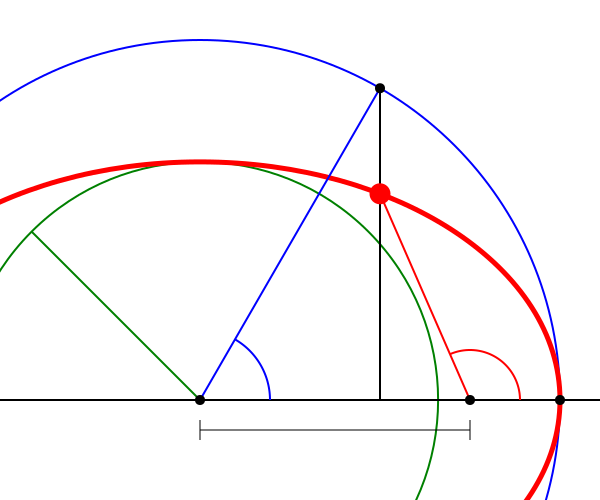
\includegraphics[width=\columnwidth]{assignment}
\caption{The eccentric anomaly of point $P$ is the angle $E$.
The center of the ellipse is point $C$, and the focus is point $F$.}
\label{fig:eccentric_anomaly}
\end{figure}

\section{Conclusions}

Hence, the eccentric anomaly is one of the parameters that determines the
position of a body on an elliptic Kepler orbit.

\section*{Acknowledgements}

I thank Wikipedia contributors for supporting the free and open encyclopedia.

%%%%%%%%%%%%%%%%%%%%%%%%%%%%%%%%%%%%%%%%%%%%%%%%%%
\section*{Data Availability}

The official MNRAS template and guide can be ontained at the
Comprehensive TeX Archive Network (CTAN) site in their directory
(\url{https://www.ctan.org/tex-archive/macros/latex/contrib/mnras}).
Sources of this file can be obtained from the Git repository
(\url{https://github.com/paveloom-university/Graphics-in-Scientific-Publications-S10-2022}).

%%%%%%%%%%%%%%%%%%%% REFERENCES %%%%%%%%%%%%%%%%%%

% The best way to enter references is to use BibTeX:

\bibliographystyle{mnras}
\bibliography{assignment} % if your bibtex file is called example.bib


% Alternatively you could enter them by hand, like this:
% This method is tedious and prone to error if you have lots of references
%\begin{thebibliography}{99}
%\bibitem[\protect\citeauthoryear{Author}{2012}]{Author2012}
%Author A.~N., 2013, Journal of Improbable Astronomy, 1, 1
%\bibitem[\protect\citeauthoryear{Others}{2013}]{Others2013}
%Others S., 2012, Journal of Interesting Stuff, 17, 198
%\end{thebibliography}

%%%%%%%%%%%%%%%%%%%%%%%%%%%%%%%%%%%%%%%%%%%%%%%%%%

%%%%%%%%%%%%%%%%% APPENDICES %%%%%%%%%%%%%%%%%%%%%

% \appendix

% \section{Some extra material}

% If you want to present additional material which would interrupt the flow of the main paper,
% it can be placed in an Appendix which appears after the list of references.

%%%%%%%%%%%%%%%%%%%%%%%%%%%%%%%%%%%%%%%%%%%%%%%%%%


% Don't change these lines
\bsp % typesetting comment
\label{lastpage}
\end{document}

% End of mnras_template.tex
